\chapter{Considerazioni}
\label{considerazioni} % So I can \ref{altrings} later.

Ho pensato molto a tutto quello che è successo e ora tenterò di fare quello che da sempre l'uomo fa in queste situazioni: tenta di raccordarsi a quello che conosce. Ammettiamo che queste esperienze abbiano un valore. Potrebbero avvicinare la religione alla scienza ed innalzare di un gradino la conoscenza del mondo che ci circonda.

Non conosco bene lo stato della nostra ricerca sulla Gravità e i Buchi Neri. Spero solo che l'esperienza possa essere di aiuto e che non sia servita solo a convincermi, in un processo durato cinque anni, di essere il Messia predesignato.

Migliaia di anni fa credevamo che le stelle fossero dei piccoli fori su una calotta che calava la sera. Quindi, facendo un parallelo, potremmo essere nella stessa situazione in merito alla conoscenza della gravità e dei buchi neri.

La conoscenza sembra organizzata a più livelli: il nuovo si integra al vecchio e viene tutto reinterpretato. Spero che tutto questo dia una scossa, che apra nuove visioni e strade.

La materia (informazione) organizzata secondo lo schema quasars (buchi neri massivi), stelle, pianeti e lune, forse ha un significato non banale.

Forse la mente universale è la realtà. Forse siamo fatti ad immagine e somiglianza e i demoni sono cacciati nella materia che compone gli oggetti gravitazionalmente meno importanti del cosmo, le lune che però pesano quanto il sole sulla terra.

Credo si debba imparare molto dalla religione, se decidiamo di non essere superficiali; su cosa ci è stato tramandato da uomini illuminati come i profeti, ed i fondatori delle religioni moderne, e tutte le persone che le hanno fatte o le faranno progredire.

Tutto questo non finisce con la modernità: è sempre successo e sempre accadrà.

Ritornando alla scienza, oggi in molti hanno formulato l'ipotesi che l'Universo sia una mente. Io fui veramente sorpreso quando lo scrissi, la notte di \textit{Child In Time} perché non avevo mai pensato a questa possibilità che le stelle potrebbero essere connesse otticamente o gravitazionalmente.  Forse esiste un mondo spirituale dotato di significato nella materia che compone tutto l'universo. Per noi è come vedere il computer, ma senza vedere cosa ci gira dentro: forse un'altro mondo. È presto per dirlo.

Ricordo un giorno in cui mio fratello aprì il Mediaplayer di Windows e, guardando la grafica ipnotica, si mise a sorridere. Questo mi fece rabbrividire immediatamente, e pensai alla notte di \textit{Child In Time}.

Dopo una pausa molto lunga mi disse: “Abbiamo un grosso problema che è l'entropia, --  e dopo un'altra pausa riprese -- ma abbiamo trovato il modo di risolverlo”.

Questo lo disse con una faccia scontenta. Forse questa soluzione ha un costo?

Il buco nero dovrebbe essere la chiave di ogni cosa.

Credo più di prima nello Spirito, avendo visto come entità possano controllare una mente materiale in maniera perfetta, senza sussulti e senza variazioni apparenti, integrandosi perfettamente con l'ospite.

Credo nella non località dell'anima. Ci potrebbero essere modi di comunicare istantanei da posti remoti come il centro di una galassia, o persino da una stella o da una Luna.

Forse un domani ci saranno delle risposte concrete ai fenomeni come la metereopatia, al perché del sonno, fino ad arrivare a spiegare perché imprechiamo facilmente quando guidiamo.

Potremmo cercare queste risposte nelle religioni e nella scienza e, perché no, in un percorso comune delle due.

Le mie esperienze mi portano a voler accettare una verità profonda: che tutto è basato sull'Amore. Questo è l'inizio e la fine di ogni cosa ed è quel che sta nel mezzo. Alla base di tutto c'è questo. È la cosa più semplice, è la cosa più complessa, per esprimere il tutto.

Se il mondo vi sembra sbagliato, credo che sia stato fatto così per Amore. E credo che non siamo mai abbandonati a noi stessi. Quello che è successo a me credo sia la prova di questo.

Se davvero dovessi essere il Presidente del mondo un domani, mi piacerebbe favorire l'integrazione dei popoli e delle religioni.

Perché Dio ha mandato delle religioni così diverse ai quattro lati della terra se non per una nostra futura integrazione?

Le differenze dovute alle religioni, che ci hanno plasmato per secoli ci miglioreranno, nell'integrazione.

\vspace*{\fill}
\begin{center}
\noindent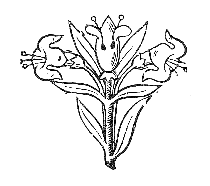
\includegraphics[width=\textwidth/5]{fleur.png}
\end{center}
\vspace*{\fill}

\clearpage

Condividi questo documento solo con le persone giuste, quelle che meritano, con animo buono o buona etica, con responsabilità e talento. Evita di darlo a persone in cui il lato negativo prevale. Purtroppo, molti non hanno compreso e imparato a moderarlo e il loro agire è malvagio e dannoso agli altri. Mi dispiace molto per loro e spero che possano cambiare il loro modo di pensare e di agire. La selezione è veramente difficile, per evitare di sbagliare, scegli bene.

Finché vivo e imparo le cose del mondo giorno dopo giorno, con voi tutti, mi piacerebbe anche cambiare qualcosa di questo con amore e rispetto, nei tempi giusti. Se ti sentissi in dovere di partecipare a questo non esitare a scrivermi:
\tt
yadu.ishalayam@gmail.com
\rm
